\documentclass[addpoints,12pt]{exam}\usepackage[]{graphicx}\usepackage[]{color}
%% maxwidth is the original width if it is less than linewidth
%% otherwise use linewidth (to make sure the graphics do not exceed the margin)
\makeatletter
\def\maxwidth{ %
  \ifdim\Gin@nat@width>\linewidth
    \linewidth
  \else
    \Gin@nat@width
  \fi
}
\makeatother

\definecolor{fgcolor}{rgb}{0.345, 0.345, 0.345}
\newcommand{\hlnum}[1]{\textcolor[rgb]{0.686,0.059,0.569}{#1}}%
\newcommand{\hlstr}[1]{\textcolor[rgb]{0.192,0.494,0.8}{#1}}%
\newcommand{\hlcom}[1]{\textcolor[rgb]{0.678,0.584,0.686}{\textit{#1}}}%
\newcommand{\hlopt}[1]{\textcolor[rgb]{0,0,0}{#1}}%
\newcommand{\hlstd}[1]{\textcolor[rgb]{0.345,0.345,0.345}{#1}}%
\newcommand{\hlkwa}[1]{\textcolor[rgb]{0.161,0.373,0.58}{\textbf{#1}}}%
\newcommand{\hlkwb}[1]{\textcolor[rgb]{0.69,0.353,0.396}{#1}}%
\newcommand{\hlkwc}[1]{\textcolor[rgb]{0.333,0.667,0.333}{#1}}%
\newcommand{\hlkwd}[1]{\textcolor[rgb]{0.737,0.353,0.396}{\textbf{#1}}}%
\let\hlipl\hlkwb


\makeatletter
\newenvironment{kframe}{%
 \def\at@end@of@kframe{}%
 \ifinner\ifhmode%
  \def\at@end@of@kframe{\end{minipage}}%
  \begin{minipage}{\columnwidth}%
 \fi\fi%
 \def\FrameCommand##1{\hskip\@totalleftmargin \hskip-\fboxsep
 \colorbox{shadecolor}{##1}\hskip-\fboxsep
     % There is no \\@totalrightmargin, so:
     \hskip-\linewidth \hskip-\@totalleftmargin \hskip\columnwidth}%
 \MakeFramed {\advance\hsize-\width
   \@totalleftmargin\z@ \linewidth\hsize
   \@setminipage}}%
 {\par\unskip\endMakeFramed%
 \at@end@of@kframe}
\makeatother

\definecolor{shadecolor}{rgb}{.97, .97, .97}
\definecolor{messagecolor}{rgb}{0, 0, 0}
\definecolor{warningcolor}{rgb}{1, 0, 1}
\definecolor{errorcolor}{rgb}{1, 0, 0}
\newenvironment{knitrout}{}{} % an empty environment to be redefined in TeX

\usepackage{alltt}
\usepackage{amsmath, amssymb}
\linespread{1.1}
\usepackage{hyperref}
\usepackage{enumerate}
\usepackage{multirow}
\usepackage{enumitem}

%-------------------DON'T CHANGE---------------------%
  %The following is needed to prevent a conflict between knitr and the exam class involving the package ``framed.''

  
  
  %This keeps images from being too big, centers them, and makes sure we use pdf images

  
  
  %Change the default width of the output to fit within the solution boxes

  %-------------------DON'T CHANGE---------------------%
  
%\printanswers

\title{Problem Set \# 13}
  \author{Econ 103}
  \date{}
\IfFileExists{upquote.sty}{\usepackage{upquote}}{}
\begin{document}
  \maketitle
  
  \section*{Lecture Progress}
  We made it to the end of the Chapter 9 slides.
  
  \section*{Homework Checklist}
  \begin{itemize}[label = $\square$]
  \item \textbf{Book Problems (Chapter 12):} 2, 3, 5, 13
  \item \textbf{Book Problems (Chapter 13):} 5, 12
  \item \textbf{Book Problems (Chapter 14):} 1, 3, 5
  \item \textbf{Additional Problems: }See below
  \item \textbf{Ask questions on Piazza}
  \item \textbf{Review slides}
  \item \textbf{Work practice exams}
  \end{itemize}
  
  
  \begin{questions}
  \item[]
  \begin{solution} \textbf{12-2}
  All of these are based on the approximation:
    $$SE(\widehat{\beta}_1) \approx \frac{\sigma}{\sqrt{n}} \cdot \frac{1}{s_X}$$
    \end{solution}
  \begin{parts}
  \item[]
  \begin{solution} \textbf{12-2(a)} Since $n$ is multiplied by four, the new SE is half as big as before. \end{solution}
  \item[]
  \begin{solution} \textbf{12-2(b)} This multiplies $s_x$ by four, so the new SE is one fourth as large as before. \end{solution}
  \item[]
  \begin{solution} \textbf{12-2(c)} Here, $n$ is divided by two, which increases the SE by a factor of $\sqrt{2}$. At the same time, however, $s_x$ increases by a factor of 2. The net effect is a decrease in SE by a factor of $\sqrt{2}$.
  \end{solution}
  \item[]
  \begin{solution} \textbf{12-2(d)} Since $\sigma^2$ is reduced by a factor two, $\sigma$ is reduced by a factor of $\sqrt{2}$. At the same time, $s_x$ increases by a factor of five. The net effect is a decrease in SE by a factor $5\sqrt{2}.$ \end{solution}
  \end{parts}
  \item[]
  \begin{solution} \textbf{13-12}
  Each of these answers refers to the following fitted regression:
    $$\begin{array}{cccccccccccccc}\widehat{S} = & 230 B& + &18A &+ &100 E& + &490 D& + &190 Y& + &50T & + & \hdots \\
  &(86)&&(8)&&(28)&&(60)&&(17)&&(370)
  \end{array}
  $$
    where the standard errors appear in parentheses below each coefficient estimate.
  \end{solution}
  \begin{parts}
  \item[]
  \begin{solution} 
  \textbf{13-12(a)}
  \begin{center}
  \begin{tabular}{lcccccc}
  &$B$ & $A$ & $E$& $D$ & $Y$& $T$\\
  \hline
  SE & 86 & 8 & 28 & 60 & 17 & 370\\
  95\% CI & $230 \pm 172$ & $18 \pm 16$ & $100 \pm 56$ & $490 \pm 120$ & $190 \pm 34$ & $50 \pm 740$ \\ 
  t ratio & 2.67&  2.25&  3.57  &8.17 &11.18 &0.14\\
  p-value &0.007& 0.024& $<0.001$& $<0.001$& $<0.001$& 0.893
  \end{tabular}
  \end{center}
  \end{solution}
  \item[]
  \begin{solution} \textbf{13-12(b)}
  We have strong evidence that each of the predictors except $T$, teaching score, is associated with higher professor salaries. The predictors that seem to be associated with the largest differences in salary are books written, PhDs supervised, and years of experience.
  \end{solution}
  \item[]
  \begin{solution} \textbf{13-12(c)}
  \begin{enumerate}
  \item FALSE. The last sentence should be changed to: ``The distribution of these estimates would be centered around the true population value.'' The point is that we do not know what the true population value is equal to: the value 230 is merely our \emph{estimate} from a particular study.
  \item FALSE. Each instance of ``one or more'' should be changed to ``one more.'' Consider two professors, A and B, who have written the sample number of ordinary articles and the same number of excellent articles, who supervise the same number of PhDs, who have the same number of years experience, and who have the same teaching score. Professor B, however, has written \emph{one more book} than Professor A. Then, we would predict that Professor B earns an average of 230 dollars more per year than Professor A.
  \item TRUE.
  \end{enumerate}
  \end{solution}
  \item[]
  \begin{solution} \textbf{13-12(d)}
  See my answer to part (ii) of (c) above. Just change the predictor that is allowed to vary by one unit and hold the others constant across professors A and B.\end{solution}
  \end{parts}
  \end{questions}
  
  
  \section*{Additional Problems}
  \begin{questions}
  
  \question This question is based on a dataset on child test scores and mother characteristics (it's referenced in the R project tips file). Before working on this question, make sure you've installed the package \texttt{arm} in RStudio. You can download the data from Professor DiTraglia's website: \begin{verbatim}www.ditraglia.com/econ103/child_test_data.csv\end{verbatim}
  The columns contained in this dataset are as follows:
  \begin{table}[h]
  \centering
  \begin{tabular}{ll}
  Variable Name & Description\\
  \hline
  \texttt{kid.score}& Child's Test Score at Age 3\\
  \texttt{mom.age}&Age of Mother at Birth of Child\\
  \texttt{mom.hs}& Mother Completed High School? (1 = Yes)\\
  \texttt{mom.iq}& Mother's IQ Score
  \end{tabular}
  \end{table}
  \begin{parts}
  \part Run a regression of \texttt{kid.score} on \texttt{mom.age}. Plot both the data and the fitted regression line, making sure to label the axes. Interpret the results. At what age do you recommend mothers give birth? What assumptions must you make to justify your recommendation?
  \begin{solution}
\begin{knitrout}
\definecolor{shadecolor}{rgb}{0.969, 0.969, 0.969}\color{fgcolor}\begin{kframe}
\begin{alltt}
\hlkwd{library}\hlstd{(arm)}
\hlstd{data.url} \hlkwb{<-} \hlstr{"http://www.ditraglia.com/econ103/child_test_data.csv"}
\hlstd{data} \hlkwb{<-} \hlkwd{read.csv}\hlstd{(data.url)}
\hlkwd{attach}\hlstd{(data)}
\hlstd{reg1} \hlkwb{<-} \hlkwd{lm}\hlstd{(kid.score} \hlopt{~} \hlstd{mom.age)}
\hlkwd{display}\hlstd{(reg1)}
\end{alltt}
\begin{verbatim}
## lm(formula = kid.score ~ mom.age)
##             coef.est coef.se
## (Intercept) 70.96     8.31  
## mom.age      0.70     0.36  
## ---
## n = 434, k = 2
## residual sd = 20.35, R-Squared = 0.01
\end{verbatim}
\begin{alltt}
\hlkwd{plot}\hlstd{(mom.age, kid.score,} \hlkwc{pch} \hlstd{=} \hlnum{20}\hlstd{,} \hlkwc{xlab} \hlstd{=} \hlstr{'Age of Mother at Birth'}\hlstd{,}
\hlkwc{ylab} \hlstd{=} \hlstr{'Child Test Score at Age 3'}\hlstd{)}
\hlkwd{coefficients}\hlstd{(reg1)}
\end{alltt}
\begin{verbatim}
## (Intercept)     mom.age 
##  70.9569209   0.6951862
\end{verbatim}
\begin{alltt}
\hlstd{intercept} \hlkwb{<-} \hlkwd{coef}\hlstd{(reg1)[}\hlnum{1}\hlstd{]}
\hlstd{slope} \hlkwb{<-} \hlkwd{coef}\hlstd{(reg1)[}\hlnum{2}\hlstd{]}
\hlkwd{abline}\hlstd{(}\hlkwc{a} \hlstd{= intercept,} \hlkwc{b} \hlstd{= slope)}
\end{alltt}
\end{kframe}

{\centering 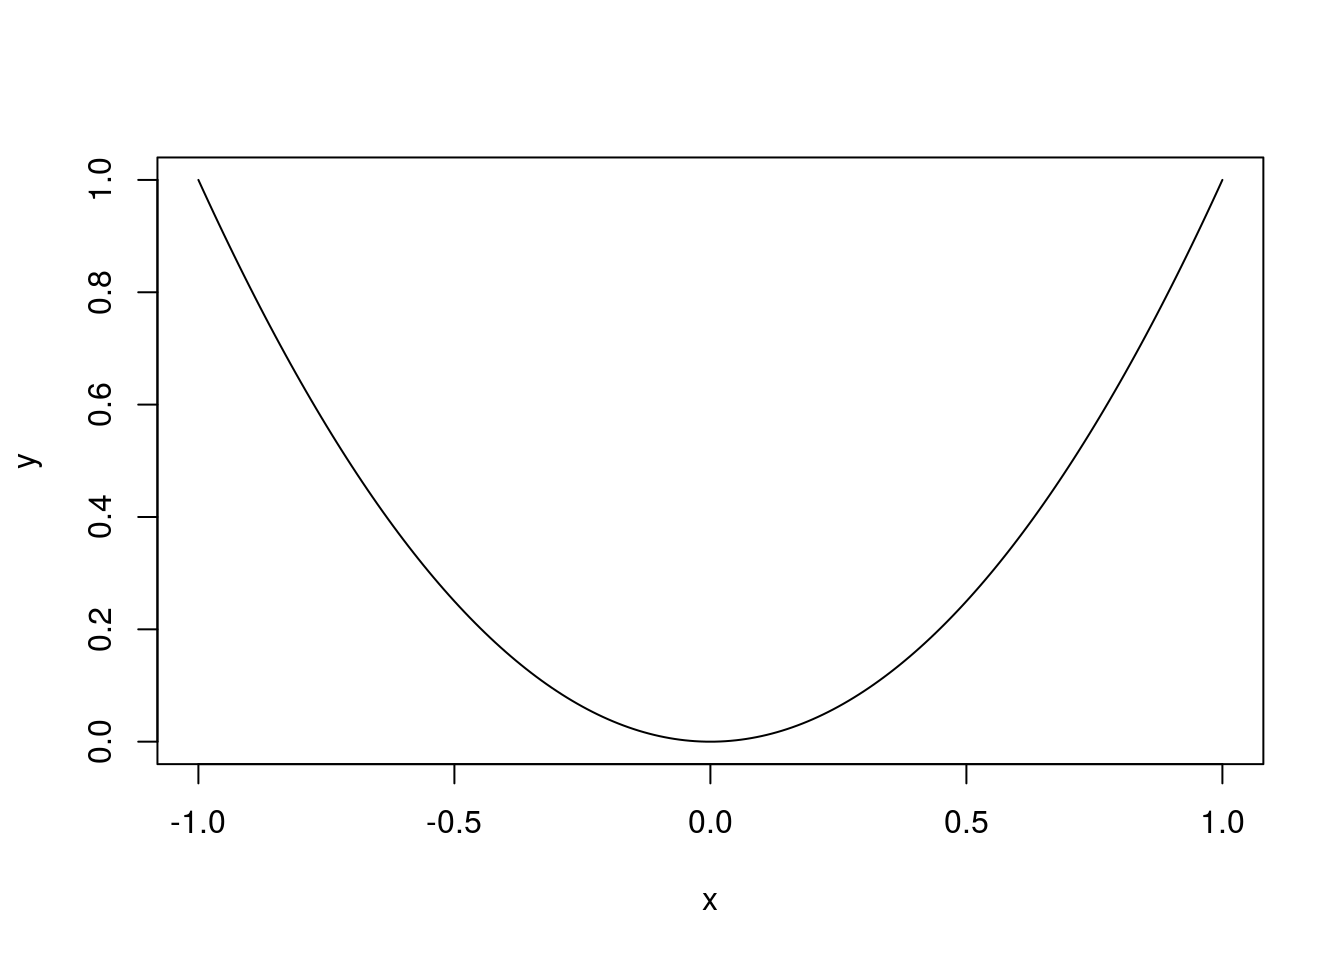
\includegraphics[width=\maxwidth]{figure/unnamed-chunk-4-1} 

}



\end{knitrout}
  Our model suggests that the children of mothers who were older when they gave birth tend to score higher. In particular, comparing two children whose mothers' age at birth differed by one year, we would predict that the child of the older mother will score, on average, 0.7 points higher. The standard error associated with the estimate, however, is fairly large. An approximate 95\% CI would just barely include zero. Nevertheless, this result is suggestive that the children of older mothers do better on the test. This would seem to suggest that women should wait to have children until they are as old as possible. However, for this advice to truly be valid, it would have to be the case that being older when you give birth \emph{caused} your child to have higher test scores. This seems unlikely. For one, we know that the incidence of birth defects (including those that affect mental ability), increases with mother's age during pregnancy. Further, teenage pregnancy is correlated with economic disadvantage and lower levels of education. There are many possible confounders here.
  \end{solution}
  \part Augment your model from part (a) by allowing a different intercept for children whose mother completed high school. Plot the data along with the regression lines for each group (those whose mother completed high school and those whose mother did not). Interpret your results and compare them to those you got in part (a).
  \begin{solution}
\begin{knitrout}
\definecolor{shadecolor}{rgb}{0.969, 0.969, 0.969}\color{fgcolor}\begin{kframe}
\begin{alltt}
\hlstd{reg2} \hlkwb{<-} \hlkwd{lm}\hlstd{(kid.score} \hlopt{~} \hlstd{mom.hs} \hlopt{+} \hlstd{mom.age)}
\hlkwd{display}\hlstd{(reg2)}
\end{alltt}
\begin{verbatim}
## lm(formula = kid.score ~ mom.hs + mom.age)
##             coef.est coef.se
## (Intercept) 70.48     8.11  
## mom.hs      11.31     2.38  
## mom.age      0.33     0.36  
## ---
## n = 434, k = 3
## residual sd = 19.86, R-Squared = 0.06
\end{verbatim}
\begin{alltt}
\hlkwd{coef}\hlstd{(reg2)}
\end{alltt}
\begin{verbatim}
## (Intercept)      mom.hs     mom.age 
##  70.4786610  11.3112315   0.3261332
\end{verbatim}
\begin{alltt}
\hlstd{slope} \hlkwb{<-} \hlkwd{coef}\hlstd{(reg2)[}\hlnum{3}\hlstd{]}
\hlstd{intercept.hs} \hlkwb{<-} \hlkwd{coef}\hlstd{(reg2)[}\hlnum{1}\hlstd{]} \hlopt{+} \hlkwd{coef}\hlstd{(reg2)[}\hlnum{2}\hlstd{]}
\hlstd{intercept.no.hs} \hlkwb{<-} \hlkwd{coef}\hlstd{(reg2)[}\hlnum{1}\hlstd{]}
\hlstd{colors} \hlkwb{<-} \hlkwd{ifelse}\hlstd{(mom.hs} \hlopt{==} \hlnum{1}\hlstd{,} \hlstr{'gray'}\hlstd{,} \hlstr{'black'}\hlstd{)}
\hlkwd{plot}\hlstd{(mom.age, kid.score, ,} \hlkwc{ylab} \hlstd{=} \hlstr{'Child Test Score at Age 3'}\hlstd{,} \hlkwc{xlab} \hlstd{=} \hlstr{'Age of Mother at Birth'}\hlstd{,} \hlkwc{pch} \hlstd{=} \hlnum{20}\hlstd{,} \hlkwc{col} \hlstd{= colors)}
\hlkwd{abline}\hlstd{(}\hlkwc{a} \hlstd{= intercept.hs,} \hlkwc{b} \hlstd{= slope,} \hlkwc{col} \hlstd{=} \hlstr{'gray'}\hlstd{)}
\hlkwd{abline}\hlstd{(}\hlkwc{a} \hlstd{= intercept.no.hs,} \hlkwc{b} \hlstd{= slope,} \hlkwc{col} \hlstd{=} \hlstr{'black'}\hlstd{)}
\end{alltt}
\end{kframe}

{\centering 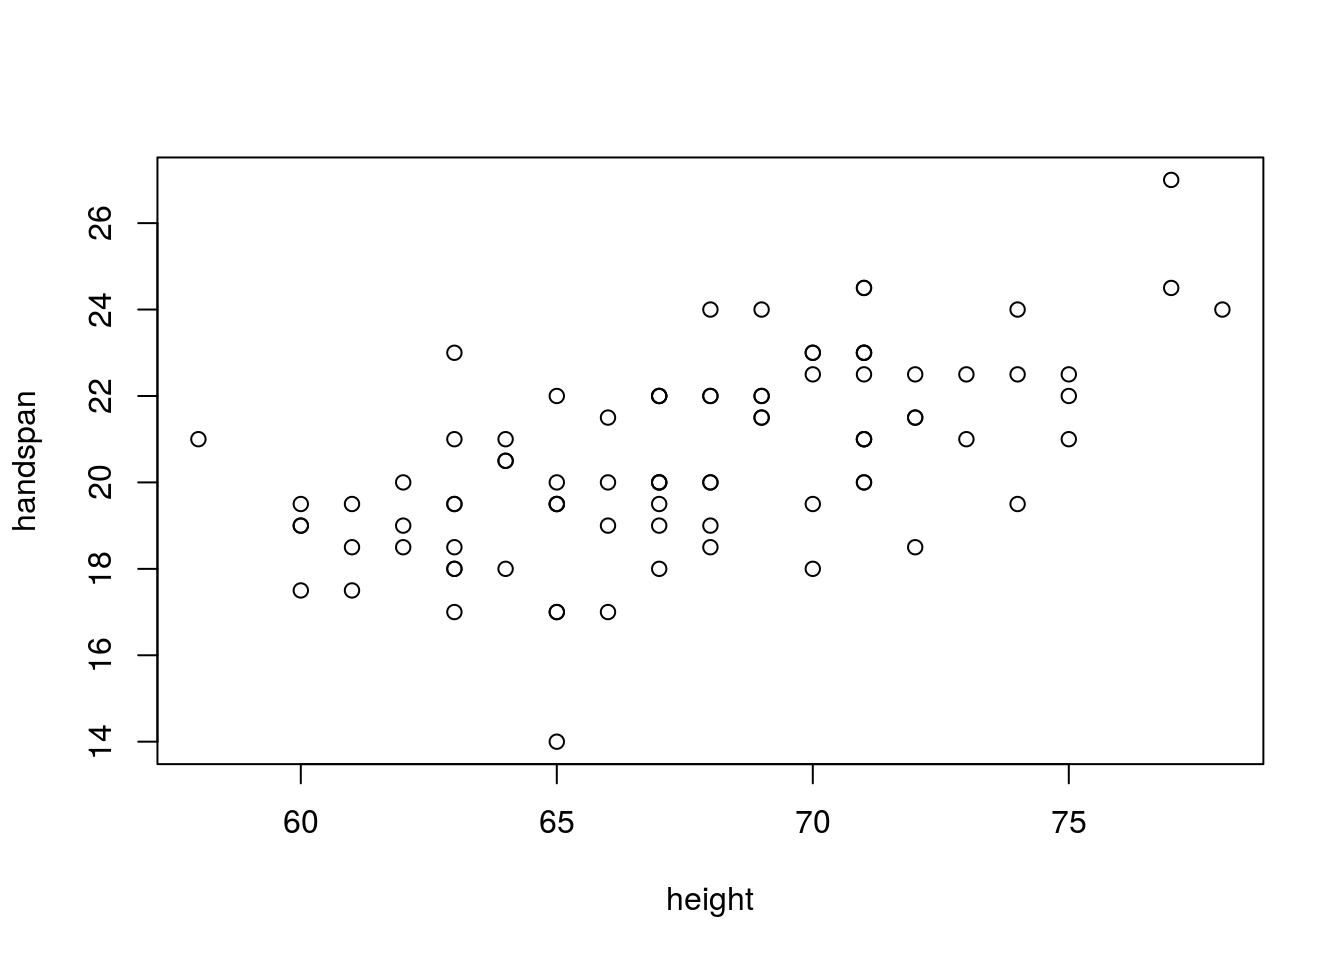
\includegraphics[width=\maxwidth]{figure/unnamed-chunk-5-1} 

}



\end{knitrout}
  By adding a dummy variable that equals one if a child's mother completed high school, we have controlled for one of the possible confounders from above: mother's level of education. We have done this by allowing the regression line to have a different intercept depending on mother's education. Comparing two children whose mothers are of the same age but only one whom attended high school, we predict that the child of the better educated mother will score, on average, 11 points higher. The standard error associated with this estimate is quite small, yielding a 95\% CI that is is nowhere near zero. We have strong evidence of a large effect from mother's education level. In contrast, once we've controlled from mother's education, the estimated effect of \texttt{mom.age} falls substantially while the associated standard error stays the same. This results in an approximate 95\% CI that includes many negative values. After controlling for mother's education, there is much less evidence to suggest that older mothers have higher-scoring children. In terms of predictive accuracy, the second model is slightly better but neither is particularly effective: we are only predicting test scores to an accuracy of about 20 points.
  \end{solution}
  \part Now allow different slopes as well as intercepts for each group (those whose mother completed high school and those whose mother did not).  Plot the data and the regression lines for each group and interpret your results. 
  \begin{solution}
\begin{knitrout}
\definecolor{shadecolor}{rgb}{0.969, 0.969, 0.969}\color{fgcolor}\begin{kframe}
\begin{alltt}
\hlstd{reg3} \hlkwb{<-} \hlkwd{lm}\hlstd{(kid.score} \hlopt{~} \hlstd{mom.hs} \hlopt{+} \hlstd{mom.age} \hlopt{+} \hlstd{mom.hs}\hlopt{:}\hlstd{mom.age)}
\hlkwd{display}\hlstd{(reg3)}
\end{alltt}
\begin{verbatim}
## lm(formula = kid.score ~ mom.hs + mom.age + mom.hs:mom.age)
##                coef.est coef.se
## (Intercept)    110.54    16.45 
## mom.hs         -41.29    18.99 
## mom.age         -1.52     0.75 
## mom.hs:mom.age   2.39     0.86 
## ---
## n = 434, k = 4
## residual sd = 19.70, R-Squared = 0.07
\end{verbatim}
\begin{alltt}
\hlkwd{coef}\hlstd{(reg3)}
\end{alltt}
\begin{verbatim}
##    (Intercept)         mom.hs        mom.age mom.hs:mom.age 
##     110.541718     -41.287465      -1.522014       2.391098
\end{verbatim}
\begin{alltt}
\hlstd{intercept.no.hs} \hlkwb{<-} \hlkwd{coef}\hlstd{(reg3)[}\hlnum{1}\hlstd{]}
\hlstd{intercept.hs} \hlkwb{<-} \hlkwd{coef}\hlstd{(reg3)[}\hlnum{1}\hlstd{]} \hlopt{+} \hlkwd{coef}\hlstd{(reg3)[}\hlnum{2}\hlstd{]}
\hlstd{slope.no.hs} \hlkwb{<-} \hlkwd{coef}\hlstd{(reg3)[}\hlnum{3}\hlstd{]}
\hlstd{slope.hs} \hlkwb{<-} \hlkwd{coef}\hlstd{(reg3)[}\hlnum{3}\hlstd{]} \hlopt{+} \hlkwd{coef}\hlstd{(reg3)[}\hlnum{4}\hlstd{]}
\hlkwd{plot}\hlstd{(mom.age, kid.score,} \hlkwc{xlab} \hlstd{=} \hlstr{'Age of Mother at Birth'}\hlstd{,} \hlkwc{pch} \hlstd{=} \hlnum{20}\hlstd{,} \hlkwc{col} \hlstd{= colors,} \hlkwc{ylab} \hlstd{=} \hlstr{'Child Test Score at Age 3'}\hlstd{)}
\hlkwd{abline}\hlstd{(}\hlkwc{a} \hlstd{= intercept.hs,} \hlkwc{b} \hlstd{= slope.hs,} \hlkwc{col} \hlstd{=} \hlstr{'gray'}\hlstd{)}
\hlkwd{abline}\hlstd{(}\hlkwc{a} \hlstd{= intercept.no.hs,} \hlkwc{b} \hlstd{= slope.no.hs,} \hlkwc{col} \hlstd{=} \hlstr{'black'}\hlstd{)}
\end{alltt}
\end{kframe}

{\centering 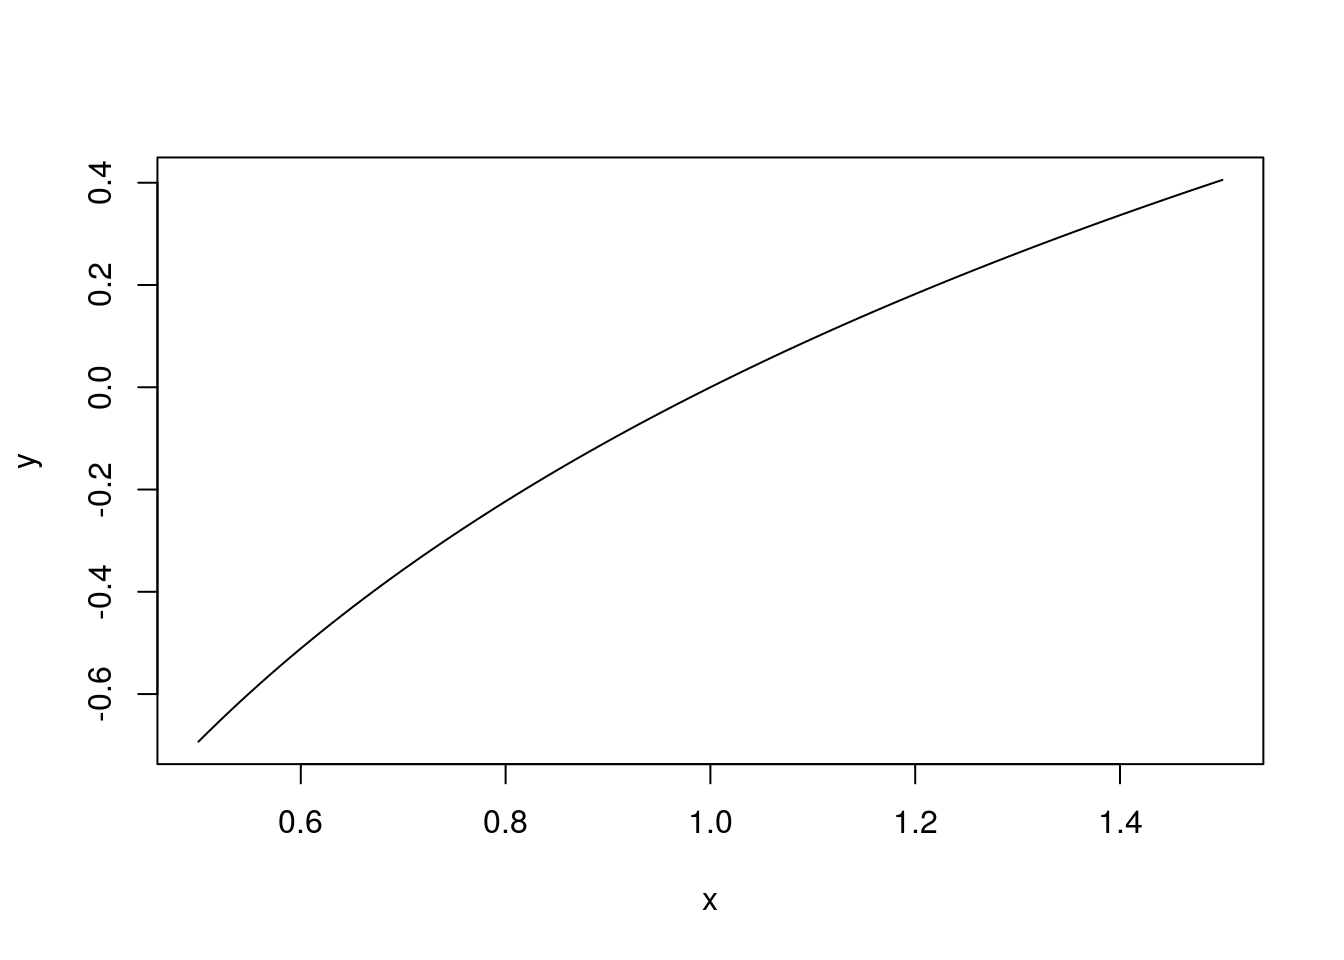
\includegraphics[width=\maxwidth]{figure/unnamed-chunk-6-1} 

}



\end{knitrout}
  This is very interesting! When we allow for different slopes as well as intercepts, by adding an \emph{interaction} between \texttt{mom.hs} and \texttt{mom.hs}, namely \texttt{mom.hs:mom.age}, we find very different results depending on mother's education. (There is strong evidence that we should allow for different slopes, since the approximate 95\% CI for the interaction does not include zero.)  For children whose mothers attended high school, there is a \emph{positive} relationship between mother's age at birth and child's test score. For children whose mothers did not attend high school, the relationship is \emph{negative}. For children whose mothers were 18 then they gave birth, there is essentially \emph{no} impact from mother's education level. As age of mother at birth increases, the impact of mother's education widens. 
  \end{solution}
  \end{parts}
  
  
  \question This example is based on 12-1 from WW4, but has been adapted somewhat for you to carry out in R. Suppose that the following expression gives the true relationship, i.e.\ the long-run average, between corn yield in tons per acre ($Y$) and the amount of fertilizer used in hundreds of pounds per acre ($X$)
  $$Y = 2.40 + 0.30 X$$
    This means that the population regression parameters are $\beta_0 = 2.40$ and $\beta_1 = 0.30$. Normally we don't know these parameters but rather use data to estimate them. In this question, however, we will pretend that we know these parameters and carry out a Monte Carlo simulation to understand how sampling variability works in the context of regression.
  \begin{parts}
  \part Write an R function called \texttt{y.plus.noise} that takes as its input a vector \texttt{x} of $X$-values and returns the corresponding $Y$ values from the above equation \emph{plus a standard normal error term}. The error term should be a \emph{different} random number for each element. 
  \begin{solution}
\begin{knitrout}
\definecolor{shadecolor}{rgb}{0.969, 0.969, 0.969}\color{fgcolor}\begin{kframe}
\begin{alltt}
\hlstd{y.plus.noise} \hlkwb{<-} \hlkwa{function}\hlstd{(}\hlkwc{x}\hlstd{)\{}
\hlnum{2.4} \hlopt{+} \hlnum{0.3} \hlopt{*} \hlstd{x} \hlopt{+} \hlkwd{rnorm}\hlstd{(}\hlkwd{length}\hlstd{(x))}
\hlstd{\}}
\end{alltt}
\end{kframe}
\end{knitrout}
  \end{solution}
  \part Define \texttt{x.test <- 0:12}, a vector containing all the integers from 0 to 12. Test our your function from part (a) by inputting \texttt{x.test} and assigning the result to \texttt{y.sim}. Make a plot of the function $Y = 2.40 + 0.30 X$ along with the points \texttt{x.test} and \texttt{y.sim}. Try repeating this: you should get a different result because the error terms are \emph{random}.
  \begin{solution}
\begin{knitrout}
\definecolor{shadecolor}{rgb}{0.969, 0.969, 0.969}\color{fgcolor}\begin{kframe}
\begin{alltt}
\hlstd{x.test} \hlkwb{<-} \hlnum{0}\hlopt{:}\hlnum{12}
\hlstd{y.sim} \hlkwb{<-} \hlkwd{y.plus.noise}\hlstd{(x.test)}
\hlkwd{plot}\hlstd{(x.test,} \hlnum{2.4} \hlopt{+} \hlnum{0.3} \hlopt{*} \hlstd{x.test,} \hlkwc{type} \hlstd{=} \hlstr{'l'}\hlstd{,} \hlkwc{xlab} \hlstd{=} \hlstr{'X'}\hlstd{,} \hlkwc{ylab} \hlstd{=} \hlstr{'Y'}\hlstd{)}
\hlkwd{points}\hlstd{(x.test, y.sim)}
\end{alltt}
\end{kframe}

{\centering 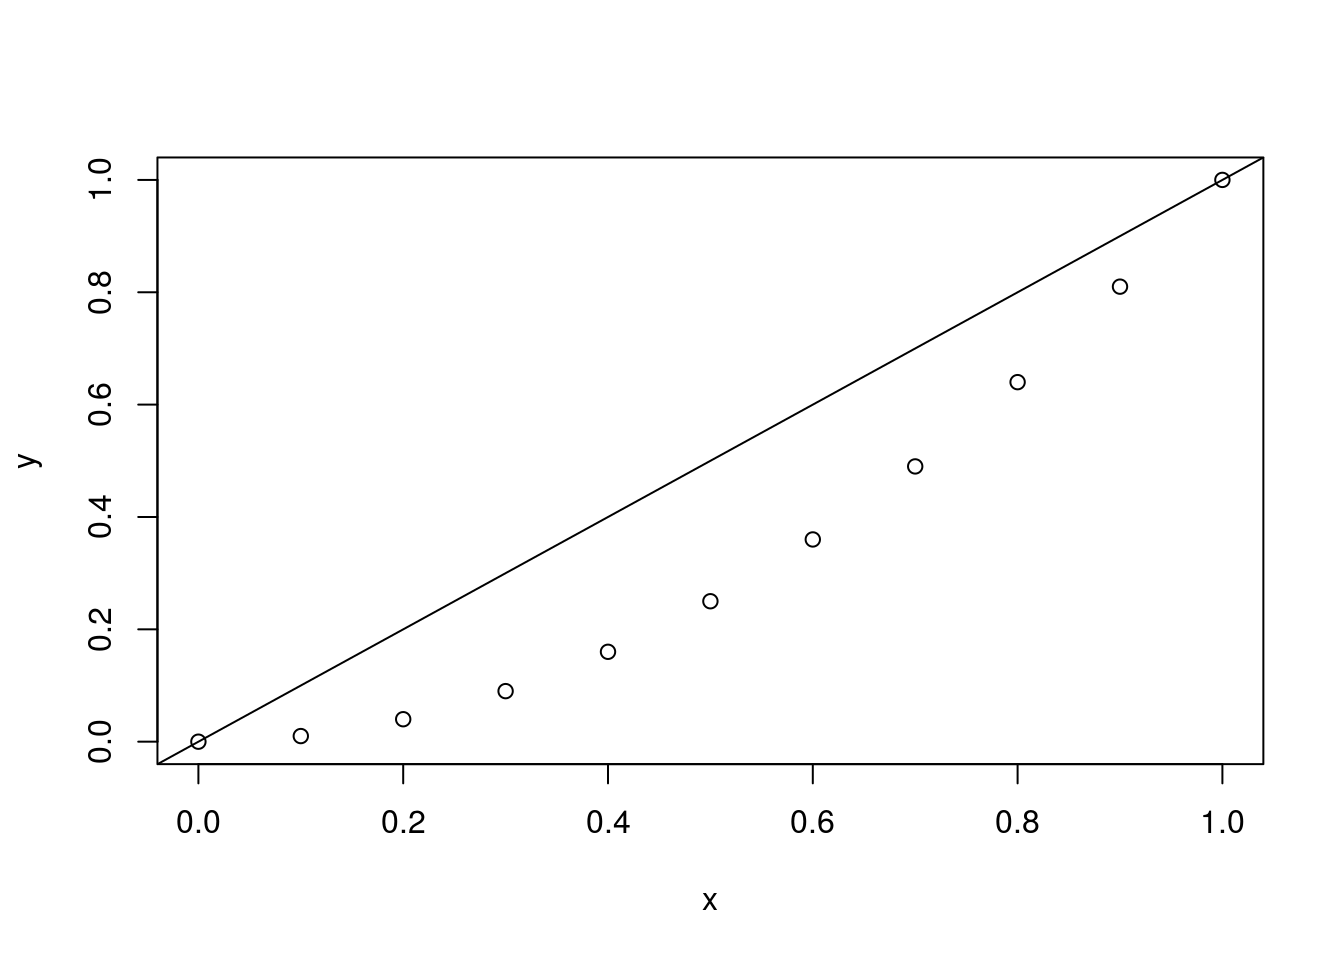
\includegraphics[width=\maxwidth]{figure/unnamed-chunk-8-1} 

}



\end{knitrout}
  Running it a second time:
\begin{knitrout}
\definecolor{shadecolor}{rgb}{0.969, 0.969, 0.969}\color{fgcolor}\begin{kframe}
\begin{alltt}
\hlstd{y.sim} \hlkwb{<-} \hlkwd{y.plus.noise}\hlstd{(x.test)}
\hlkwd{plot}\hlstd{(x.test,} \hlnum{2.4} \hlopt{+} \hlnum{0.3} \hlopt{*} \hlstd{x.test,} \hlkwc{type} \hlstd{=} \hlstr{'l'}\hlstd{,} \hlkwc{xlab} \hlstd{=} \hlstr{'X'}\hlstd{,} \hlkwc{ylab} \hlstd{=} \hlstr{'Y'}\hlstd{)}
\hlkwd{points}\hlstd{(x.test, y.sim)}
\end{alltt}
\end{kframe}

{\centering 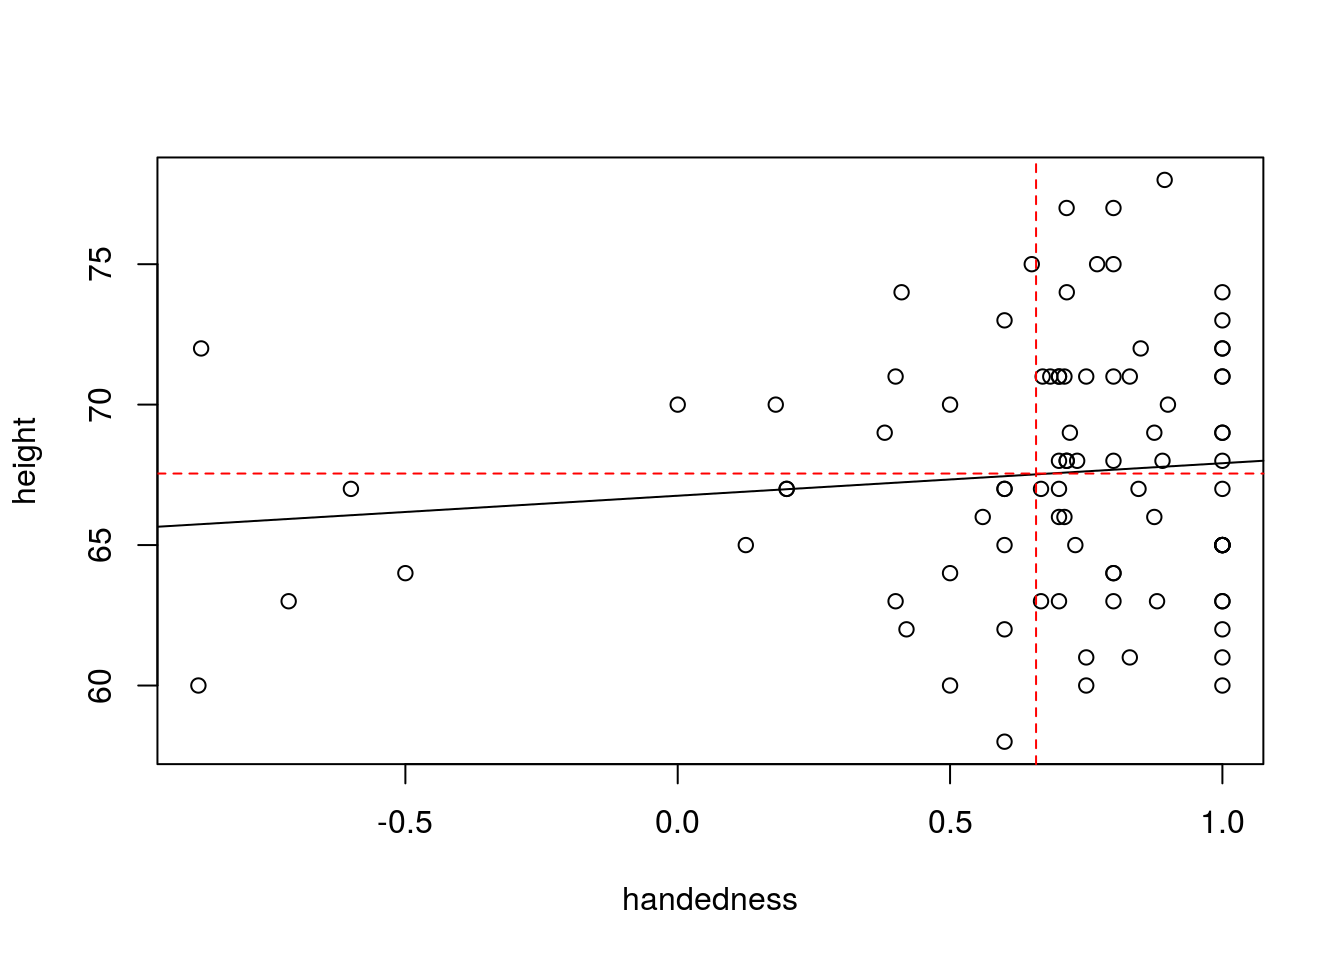
\includegraphics[width=\maxwidth]{figure/unnamed-chunk-9-1} 

}



\end{knitrout}
  \end{solution}
  \part Run a regression of \texttt{y.sim} on \texttt{x.test} using the R command \texttt{lm(y.sim ~ x.test)}. Compare the estimated coefficients to the population regression parameters from above by adding the \emph{fitted} regression line to your plot from part (b) using code similar to the following:
  \begin{verbatim}
  reg <- lm(y.sim ~ x.test)
  estimates <- coefficients(reg)
  a.estimate <- estimates[1]
  b.estimate <- estimates[2]
  abline(a = a.estimate, b = b.estimate, lty = 2)
  \end{verbatim}
  The command \texttt{coefficients} extracts the estimated regression coefficients as a numeric vector, while \texttt{abline} plots a line based on its intercept ($a$) and slope ($b$). Setting the parameter \texttt{lty = 2} gives a dashed line. If you repeat part (b) followed by part (c) what changes in the picture and what stays the same?
  \begin{solution}
\begin{knitrout}
\definecolor{shadecolor}{rgb}{0.969, 0.969, 0.969}\color{fgcolor}\begin{kframe}
\begin{alltt}
\hlkwd{lm}\hlstd{(y.sim} \hlopt{~} \hlstd{x.test)}
\end{alltt}
\begin{verbatim}
## 
## Call:
## lm(formula = y.sim ~ x.test)
## 
## Coefficients:
## (Intercept)       x.test  
##      2.6319       0.2766
\end{verbatim}
\begin{alltt}
\hlstd{estimates} \hlkwb{<-} \hlkwd{coefficients}\hlstd{(}\hlkwd{lm}\hlstd{(y.sim} \hlopt{~} \hlstd{x.test))}
\hlstd{a.estimate} \hlkwb{<-} \hlstd{estimates[}\hlnum{1}\hlstd{]}
\hlstd{b.estimate} \hlkwb{<-} \hlstd{estimates[}\hlnum{2}\hlstd{]}
\hlkwd{plot}\hlstd{(x.test,} \hlnum{2.4} \hlopt{+} \hlnum{0.3} \hlopt{*} \hlstd{x.test,} \hlkwc{type} \hlstd{=} \hlstr{'l'}\hlstd{,} \hlkwc{xlab} \hlstd{=} \hlstr{'X'}\hlstd{,} \hlkwc{ylab} \hlstd{=} \hlstr{'Y'}\hlstd{)}
\hlkwd{points}\hlstd{(x.test, y.sim)}
\hlkwd{abline}\hlstd{(}\hlkwc{a} \hlstd{= a.estimate,} \hlkwc{b} \hlstd{= b.estimate,} \hlkwc{lty} \hlstd{=} \hlnum{2}\hlstd{,} \hlkwc{col} \hlstd{=} \hlstr{'red'}\hlstd{)}
\end{alltt}
\end{kframe}

{\centering 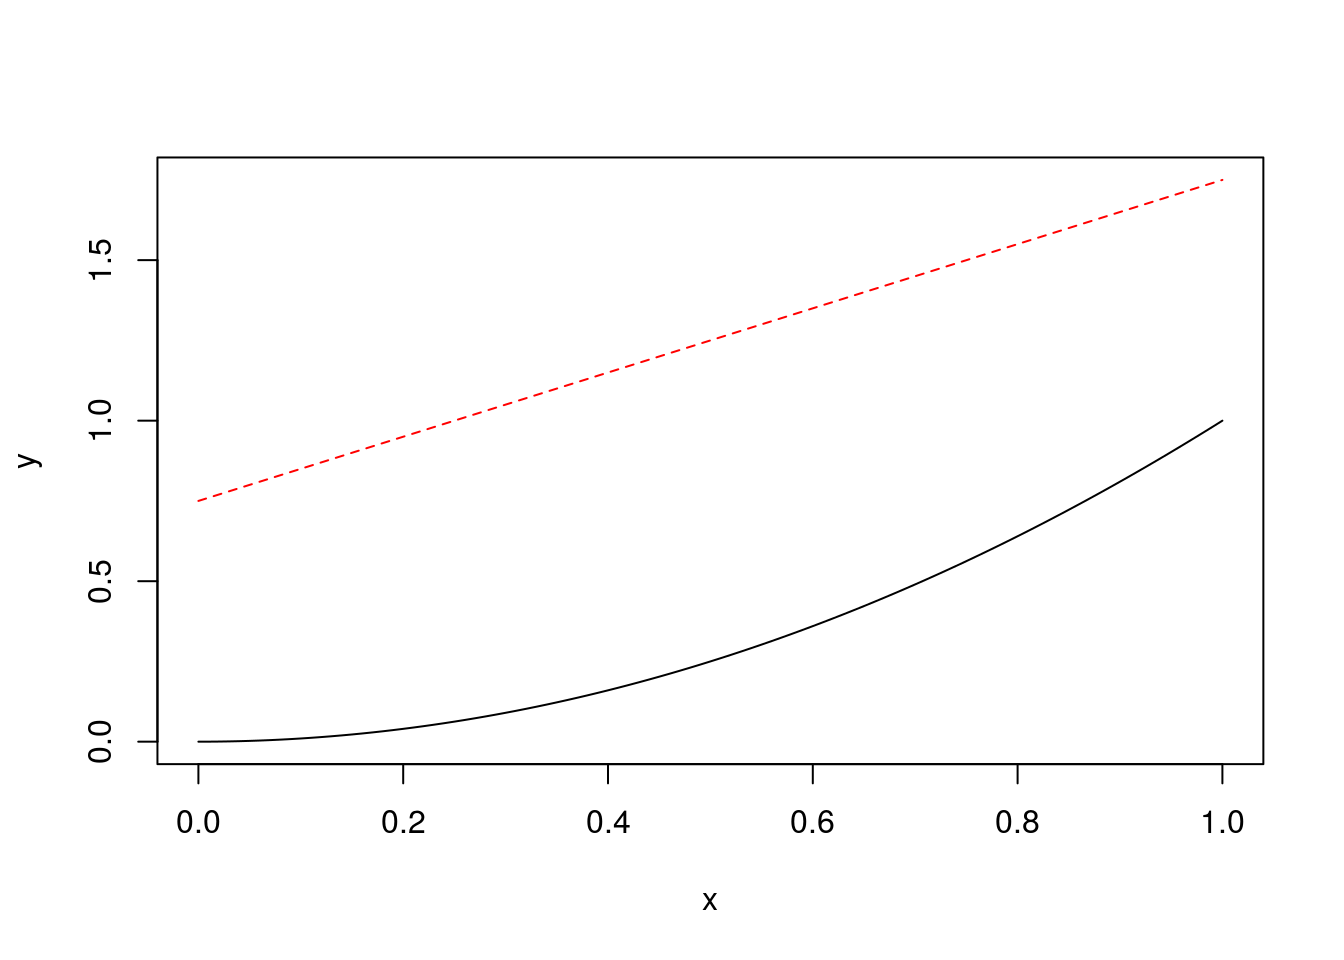
\includegraphics[width=\maxwidth]{figure/unnamed-chunk-10-1} 

}



\end{knitrout}
  Repeating this with new draws for \texttt{y.sim}, 
\begin{knitrout}
\definecolor{shadecolor}{rgb}{0.969, 0.969, 0.969}\color{fgcolor}\begin{kframe}
\begin{alltt}
\hlstd{y.sim} \hlkwb{<-} \hlkwd{y.plus.noise}\hlstd{(x.test)}
\hlstd{estimates} \hlkwb{<-} \hlkwd{coefficients}\hlstd{(}\hlkwd{lm}\hlstd{(y.sim} \hlopt{~} \hlstd{x.test))}
\hlstd{a.estimate} \hlkwb{<-} \hlstd{estimates[}\hlnum{1}\hlstd{]}
\hlstd{b.estimate} \hlkwb{<-} \hlstd{estimates[}\hlnum{2}\hlstd{]}
\hlkwd{plot}\hlstd{(x.test,} \hlnum{2.4} \hlopt{+} \hlnum{0.3} \hlopt{*} \hlstd{x.test,} \hlkwc{type} \hlstd{=} \hlstr{'l'}\hlstd{,} \hlkwc{xlab} \hlstd{=} \hlstr{'X'}\hlstd{,} \hlkwc{ylab} \hlstd{=} \hlstr{'Y'}\hlstd{)}
\hlkwd{points}\hlstd{(x.test, y.sim)}
\hlkwd{abline}\hlstd{(}\hlkwc{a} \hlstd{= a.estimate,} \hlkwc{b} \hlstd{= b.estimate,} \hlkwc{lty} \hlstd{=} \hlnum{2}\hlstd{,} \hlkwc{col} \hlstd{=} \hlstr{'red'}\hlstd{)}
\end{alltt}
\end{kframe}

{\centering 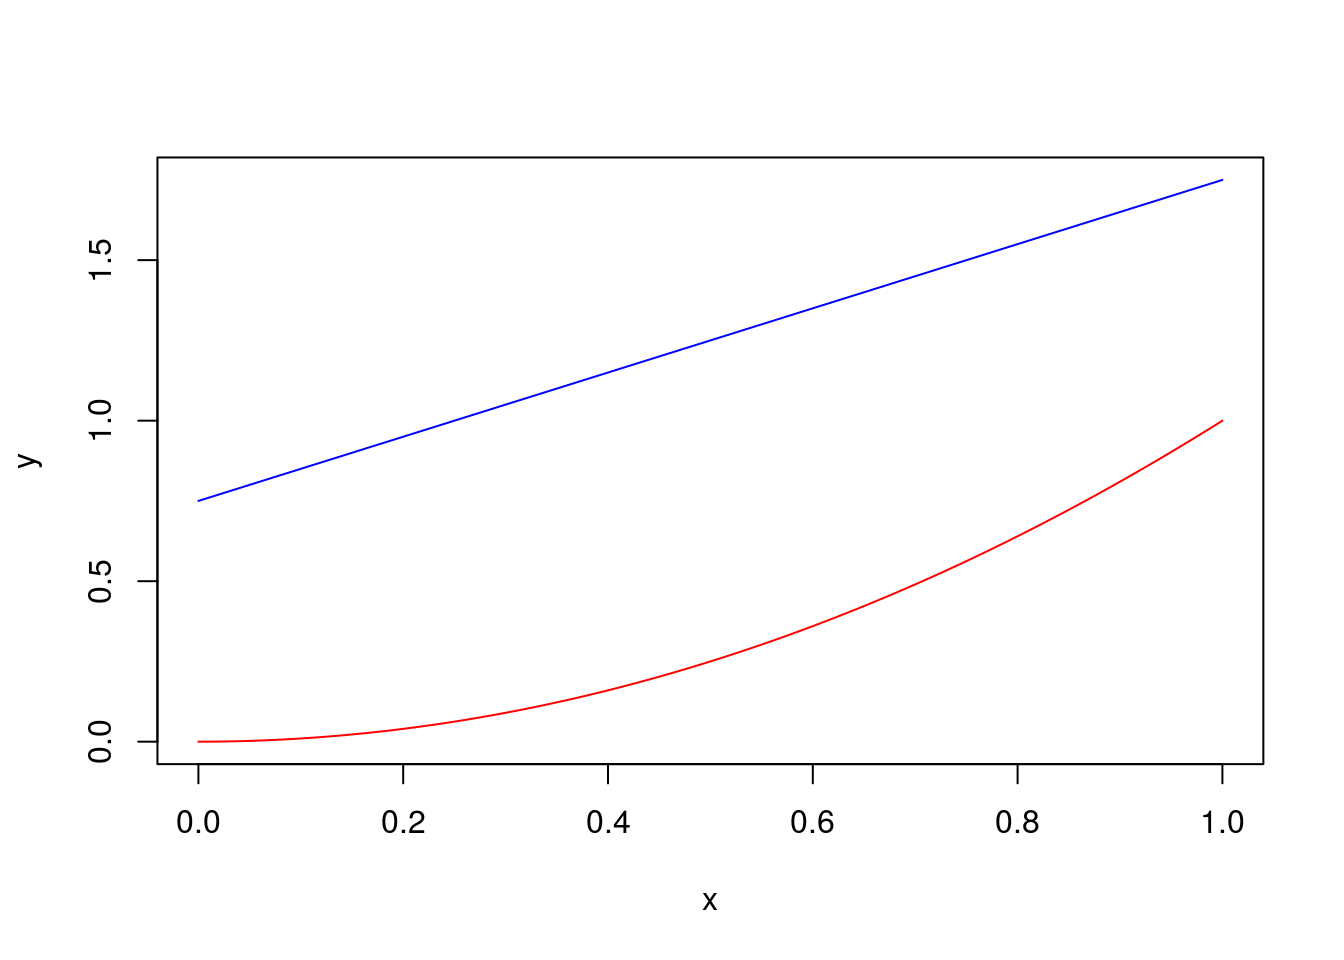
\includegraphics[width=\maxwidth]{figure/unnamed-chunk-11-1} 

}



\end{knitrout}
  In each plot the \emph{population regression line} stays the same as do the $X$-coordinates of the points. What differs each time we re-run the function \texttt{y.plus.noise} is the \emph{random errors}. This changes the $Y$-coordinates of the points and leads to a different estimated regression line. This corresponds to \emph{sampling variability}.
  \end{solution}
  \part Adapting the code from above, write a function called \texttt{slope.sim} that takes as its input a vector \texttt{x} of $X$-values and then does the following:
  \begin{itemize}
  \item[Step 1] Create a vector \texttt{y.sim} as above.
  \item[Step 2] Regress \texttt{y.sim} on \texttt{x} and call the result \texttt{reg}.
  \item[Step 3] Return the \emph{estimated slope coefficient} from \texttt{reg}.
  \end{itemize}
  \begin{solution}
\begin{knitrout}
\definecolor{shadecolor}{rgb}{0.969, 0.969, 0.969}\color{fgcolor}\begin{kframe}
\begin{alltt}
\hlstd{slope.sim} \hlkwb{<-} \hlkwa{function}\hlstd{(}\hlkwc{x}\hlstd{)\{}

\hlstd{y.sim} \hlkwb{<-} \hlnum{2.4} \hlopt{+} \hlnum{0.3} \hlopt{*} \hlstd{x} \hlopt{+} \hlkwd{rnorm}\hlstd{(}\hlkwd{length}\hlstd{(x))}
\hlstd{reg} \hlkwb{<-} \hlkwd{lm}\hlstd{(y.sim} \hlopt{~} \hlstd{x)}
\hlstd{b} \hlkwb{<-} \hlkwd{coefficients}\hlstd{(reg)[}\hlnum{2}\hlstd{]}
\hlkwd{return}\hlstd{(b)}

\hlstd{\}}
\end{alltt}
\end{kframe}
\end{knitrout}
  \end{solution}
  \part To simulate the sampling distribution of the estimated regression slope parameter using the population regression given above, use the function \texttt{replicate} to call your function \texttt{slope.sim} 1000 times and store the result in a vector called \texttt{b.sim}. In each of these replications, use \texttt{x.test} as the input for \texttt{slope.sim}. 
  \begin{solution}
\begin{knitrout}
\definecolor{shadecolor}{rgb}{0.969, 0.969, 0.969}\color{fgcolor}\begin{kframe}
\begin{alltt}
\hlstd{b.sim} \hlkwb{<-} \hlkwd{replicate}\hlstd{(}\hlnum{1000}\hlstd{,} \hlkwd{slope.sim}\hlstd{(x.test))}
\end{alltt}
\end{kframe}
\end{knitrout}
  \end{solution}
  \part Calculate the mean standard deviation of the vector \texttt{b.sim} and plot a histogram. Explain your results.
  \begin{solution}
\begin{knitrout}
\definecolor{shadecolor}{rgb}{0.969, 0.969, 0.969}\color{fgcolor}\begin{kframe}
\begin{alltt}
\hlkwd{mean}\hlstd{(b.sim)}
\end{alltt}
\begin{verbatim}
## [1] 0.3004082
\end{verbatim}
\begin{alltt}
\hlkwd{sd}\hlstd{(b.sim)}
\end{alltt}
\begin{verbatim}
## [1] 0.07333328
\end{verbatim}
\begin{alltt}
\hlkwd{hist}\hlstd{(b.sim)}
\end{alltt}
\end{kframe}

{\centering \includegraphics[width=\maxwidth]{figure/unnamed-chunk-14-1} 

}



\end{knitrout}
  We see that the sampling distribution of the estimated regression slope coefficient is centered at the population slope coefficient $\beta = 0.3$ and the sampling distribution is approximately normal. The standard error is around 0.07.
  \end{solution}
  \end{parts}	
  
  \end{questions}
  
  \end{document}
